\section{Design Front-End}
\label{sec:RequisitiFrontEnd}

Nel presente capitolo vengono riportati alcuni mockup relativi alle schermate del sito da realizzare. Queste schermate hanno l’obiettivo di rappresentare come l’applicazione si dovrà presentare all’utente finale, il front-end (FE), nel caso dei seguenti requisiti funzionali descritti precedentemente: 
\begin{itemize}
    \item registrazione e login nella piattaforma (\ref{rf:1.1});
    \item interazione con calendari di altre persone (\ref{rf:4.1}) e possibilità di avere più calendari personali (\ref{rf:4.2});
    \item compilazione/modifica evento (\ref{rf:5});
    \item inserimento impegno (\ref{rf:6});
    \item interazione con un servizio di mappe (\ref{rf:8.2});
    \item riorganizzazione di attività (\ref{rf:10});
    \item informazioni sull’uso del tempo (\ref{rf:9});
    \item recupero password (\ref{rf:15}) % per questo non so se ha senso metterlo, più che altro perché c'è solo quella riga di recupero e non tutta la procedura.
\end{itemize}

\begin{listaPersonale}{FE}
    \elemento[LOGIN NELLA PIATTAFORMA]{fe:1} In questa \href{https://www.figma.com/proto/cO66hx25OizBABGtWp8XlT/Planify?node-id=82%3A74&scaling=scale-down&page-id=0%3A1&starting-point-node-id=25%3A82}{schermata}, l’utente già registrato mediante email e password, deve inserire le credenziali da lui scelte per accedere al sito. Invece, coloro che hanno fatto accesso grazie all’utilizzo di servizi di terze parti, devono proseguire la loro autenticazione premendo il tasto corrispondente al servizio esterno da loro utilizzato per registrarsi (\ref{rf:1.1}). Sbagliando più volte la password del proprio account si ottiene la \href{https://www.figma.com/proto/cO66hx25OizBABGtWp8XlT/Planify?node-id=266%3A875&scaling=scale-down&page-id=0%3A1&starting-point-node-id=25%3A82}{schermata} in "Figura 1.1". %facendo ref mi viene 2, dovrei fare un altro comando per fare il giusto riferimento 
    Se l’utente non si è ancora registrato sul sito deve schiacciare “Registrati” oppure proseguire l’autenticazione con il servizio di terze parti offerto, ovvero Google. \\ \\
    \begin{figure}[H]
        \centering
        \href{https://www.figma.com/proto/cO66hx25OizBABGtWp8XlT/Planify?node-id=82%3A74&scaling=scale-down&page-id=0%3A1&starting-point-node-id=25%3A82}{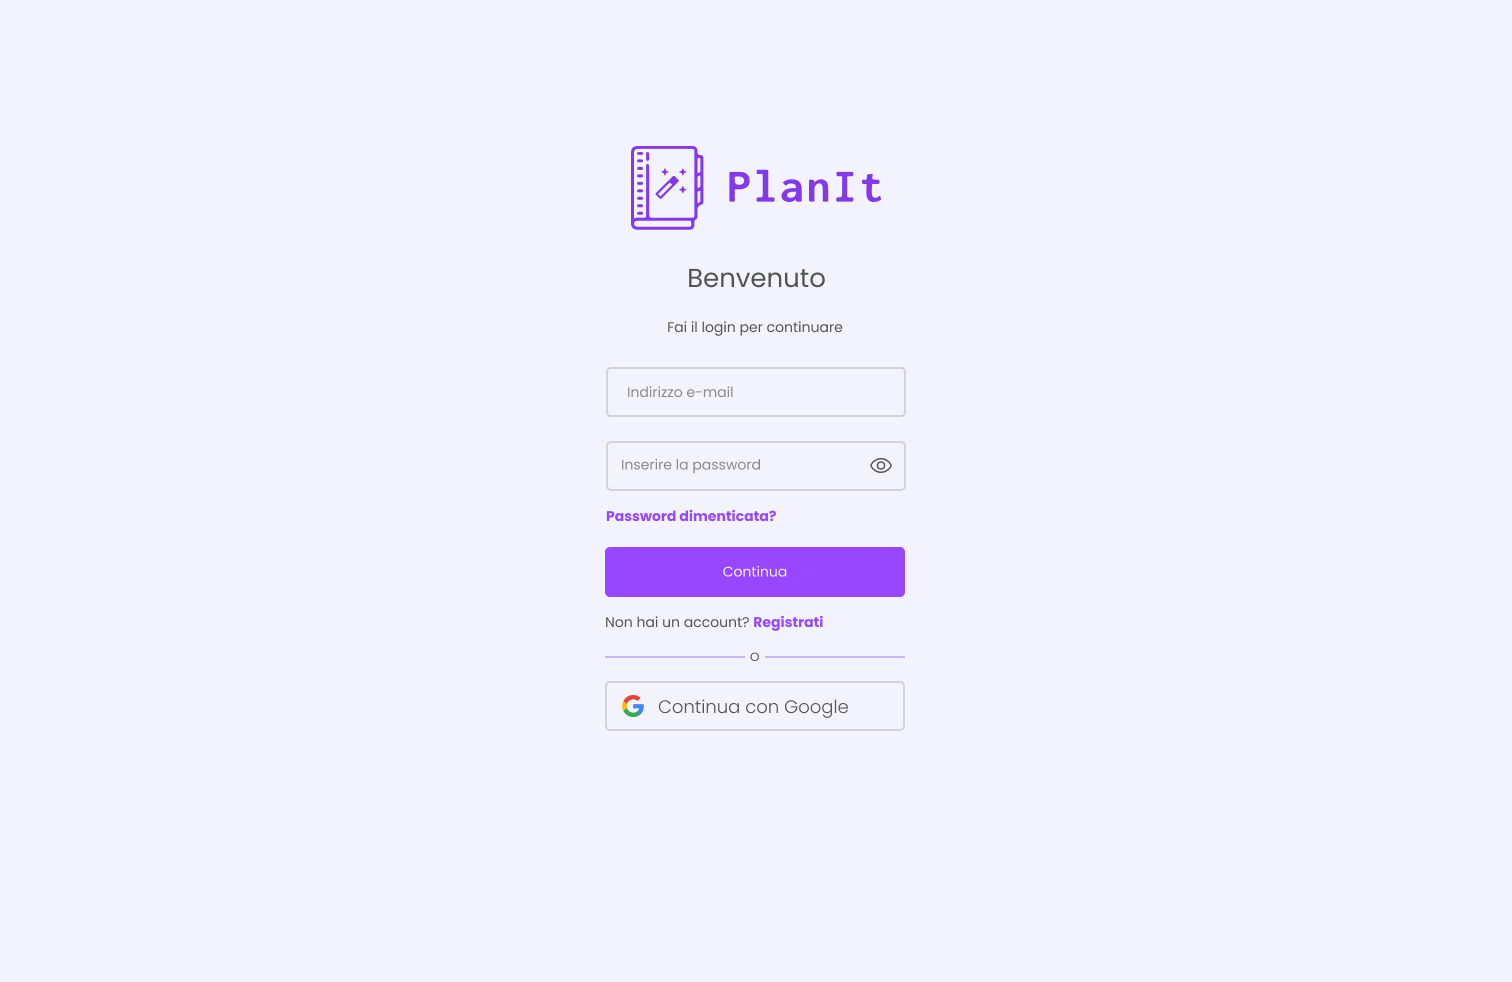
\includegraphics[width=1\textwidth]{img/FrontEnd/Login.png}}
        \caption{Figura 1: schermata quando si apre il sito PlanIt}
    \end{figure}
    \begin{listaPersonale2}{FE}
        \elemento[SCHERMATA RESET PASSWORD]{fe:1.1}
        \begin{figure}[H]
            \centering
            \href{https://www.figma.com/proto/cO66hx25OizBABGtWp8XlT/Planify?node-id=266%3A875&scaling=scale-down&page-id=0%3A1&starting-point-node-id=25%3A82}{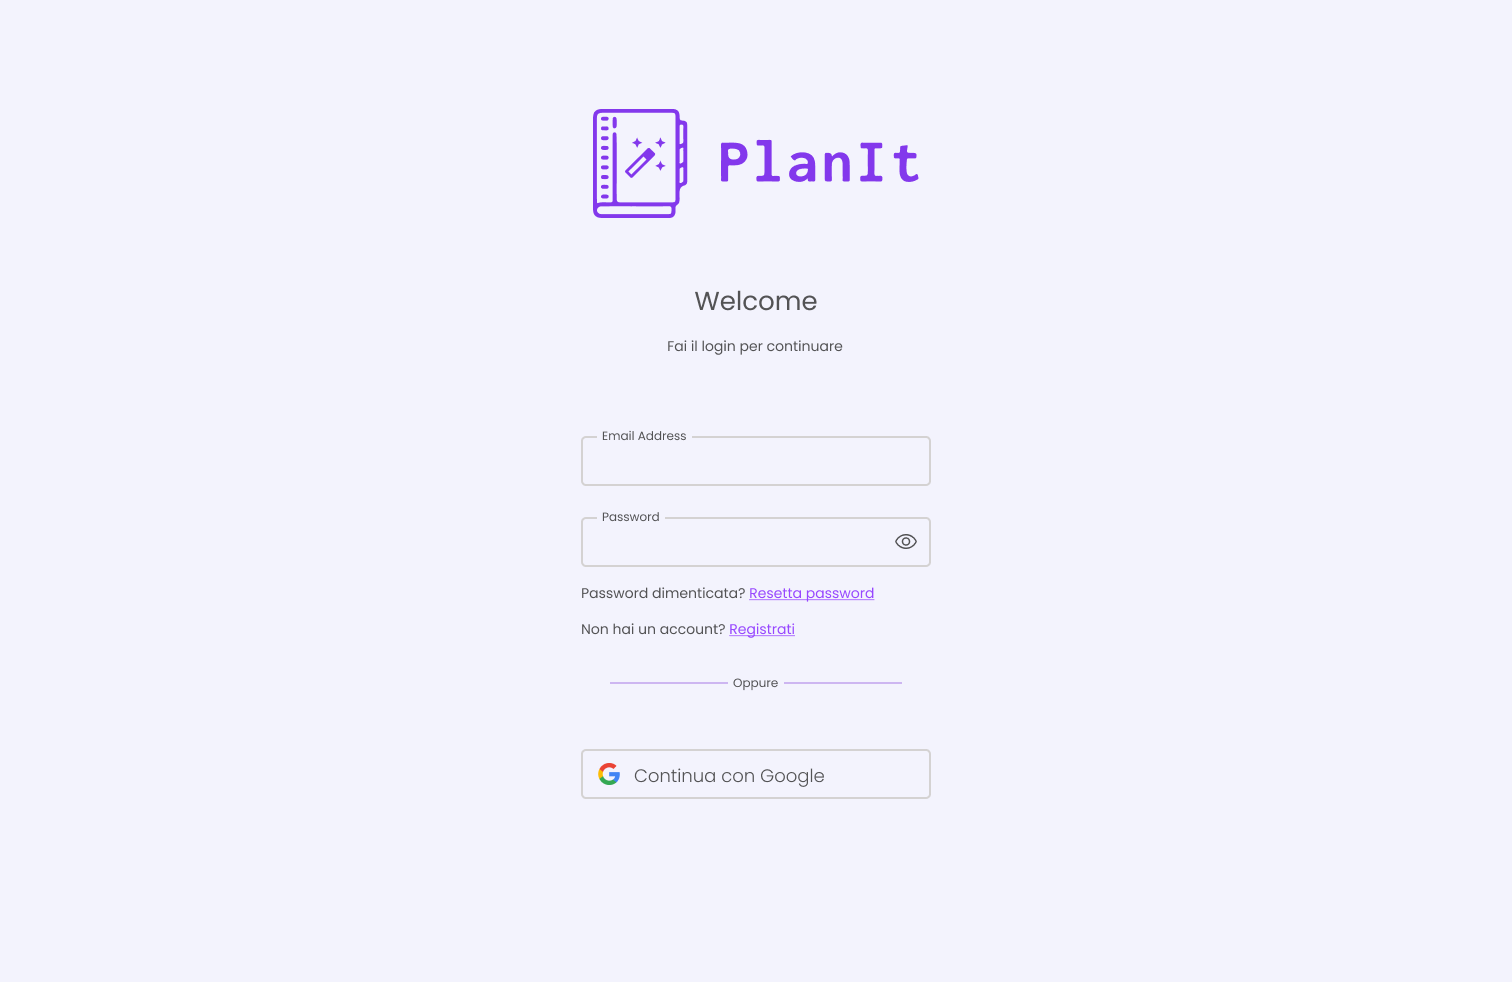
\includegraphics[width=1\textwidth]{img/FrontEnd/ResettaPssw.png}}
            \caption{Figura 1.1: schermata che appare quando si sbaglia più volte una password}
        \end{figure}

        \begin{comment}\begin{figure}%[5]
            \href{https://www.figma.com/proto/cO66hx25OizBABGtWp8XlT/Planify?node-id=266%3A875&scaling=scale-down&page-id=0%3A1&starting-point-node-id=25%3A82}{%
                \parbox{\textwidth}{
                    \centering
                    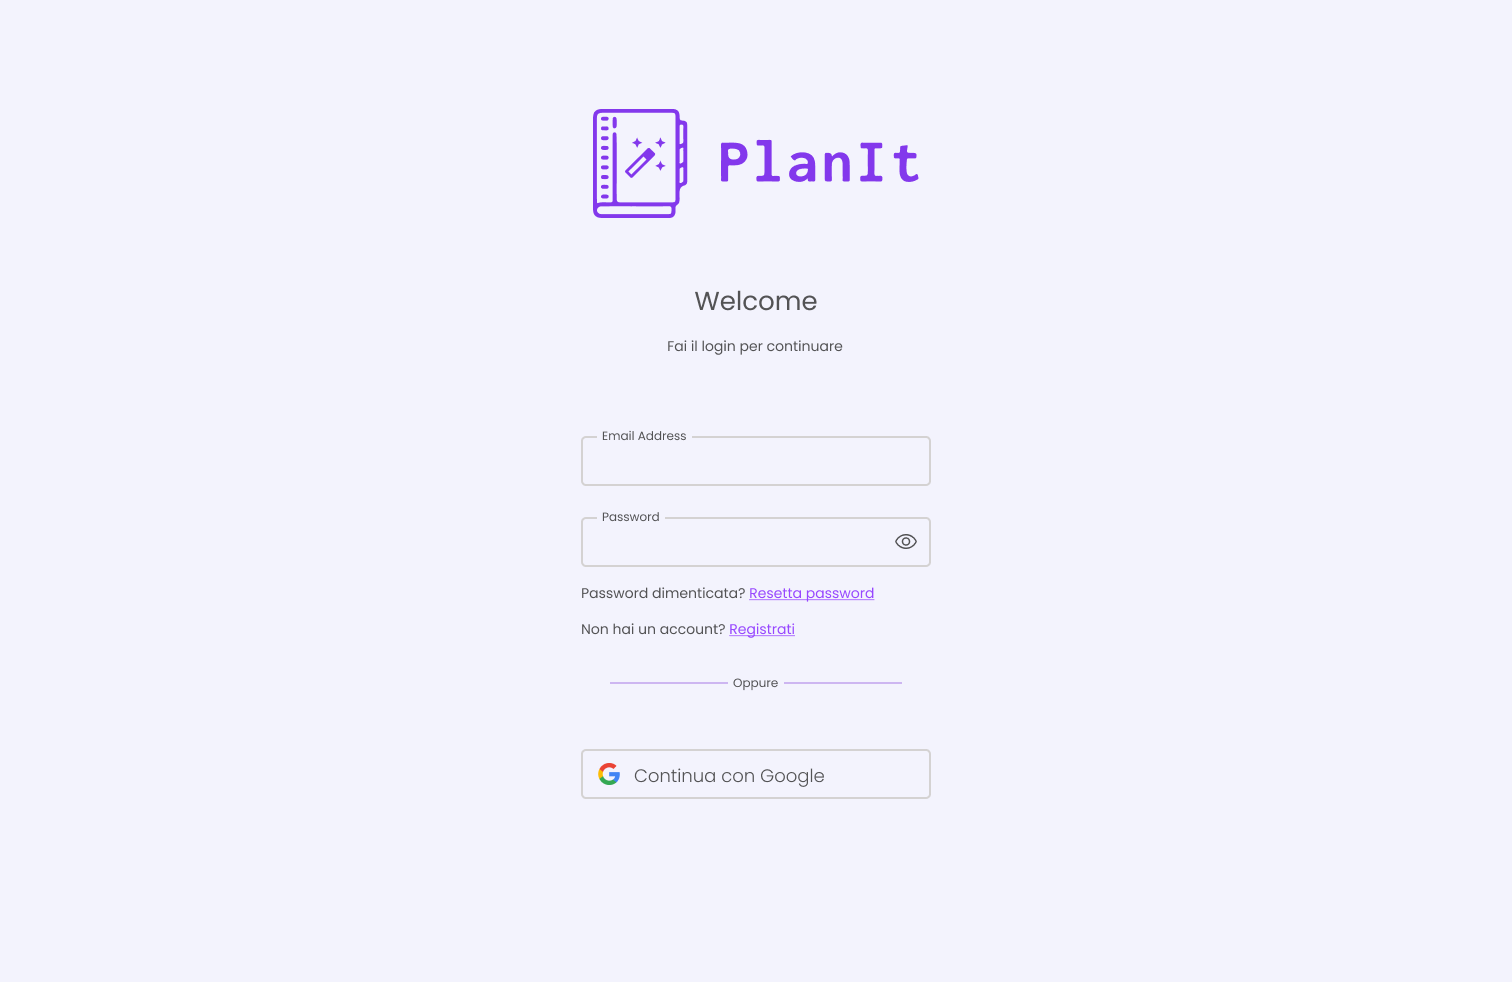
\includegraphics[width=1\textwidth]{img/FrontEnd/ResettaPssw.png}
                    \caption{Figura 1.1: schermata che appare quando si sbaglia più volte una password}
                }
            }
        \end{figure}
        \end{comment}

    \end{listaPersonale2}

    \pagebreak%quasi quasi metterei un pagebreak per ciascuna schermata così per renderlo più ordinato
    
    \elemento [SCHERMATA PRINCIPALE] {fe:2} Questa \href{https://www.figma.com/proto/cO66hx25OizBABGtWp8XlT/Planify?node-id=25%3A82&scaling=scale-down&page-id=0%3A1&starting-point-node-id=25%3A82}{schermata} è la schermata principale della piattaforma PlanIt. L’utente, dopo aver fatto l’accesso al sito oppure proseguito con la modalità demo, giungerà a questa pagina, dove potrà guardare gli eventi posti nella settimana. L’utente ha la possibilità, dal menù al di sopra del calendario, di spostarsi di data sia in mesi che in settimane, visualizzare il calendario per settimana, mese ed anno e accedere agli altri calendari personali e a quelli condivisi (\ref{rf:4.1}). Infine è presente anche il bottone "+” con cui si accede al pop-up di compilazione/aggiunta evento(\ref{rf:5}).
    \begin{figure}[H]
        \centering
        \href{https://www.figma.com/proto/cO66hx25OizBABGtWp8XlT/Planify?node-id=25%3A82&scaling=scale-down&page-id=0%3A1&starting-point-node-id=25%3A82}{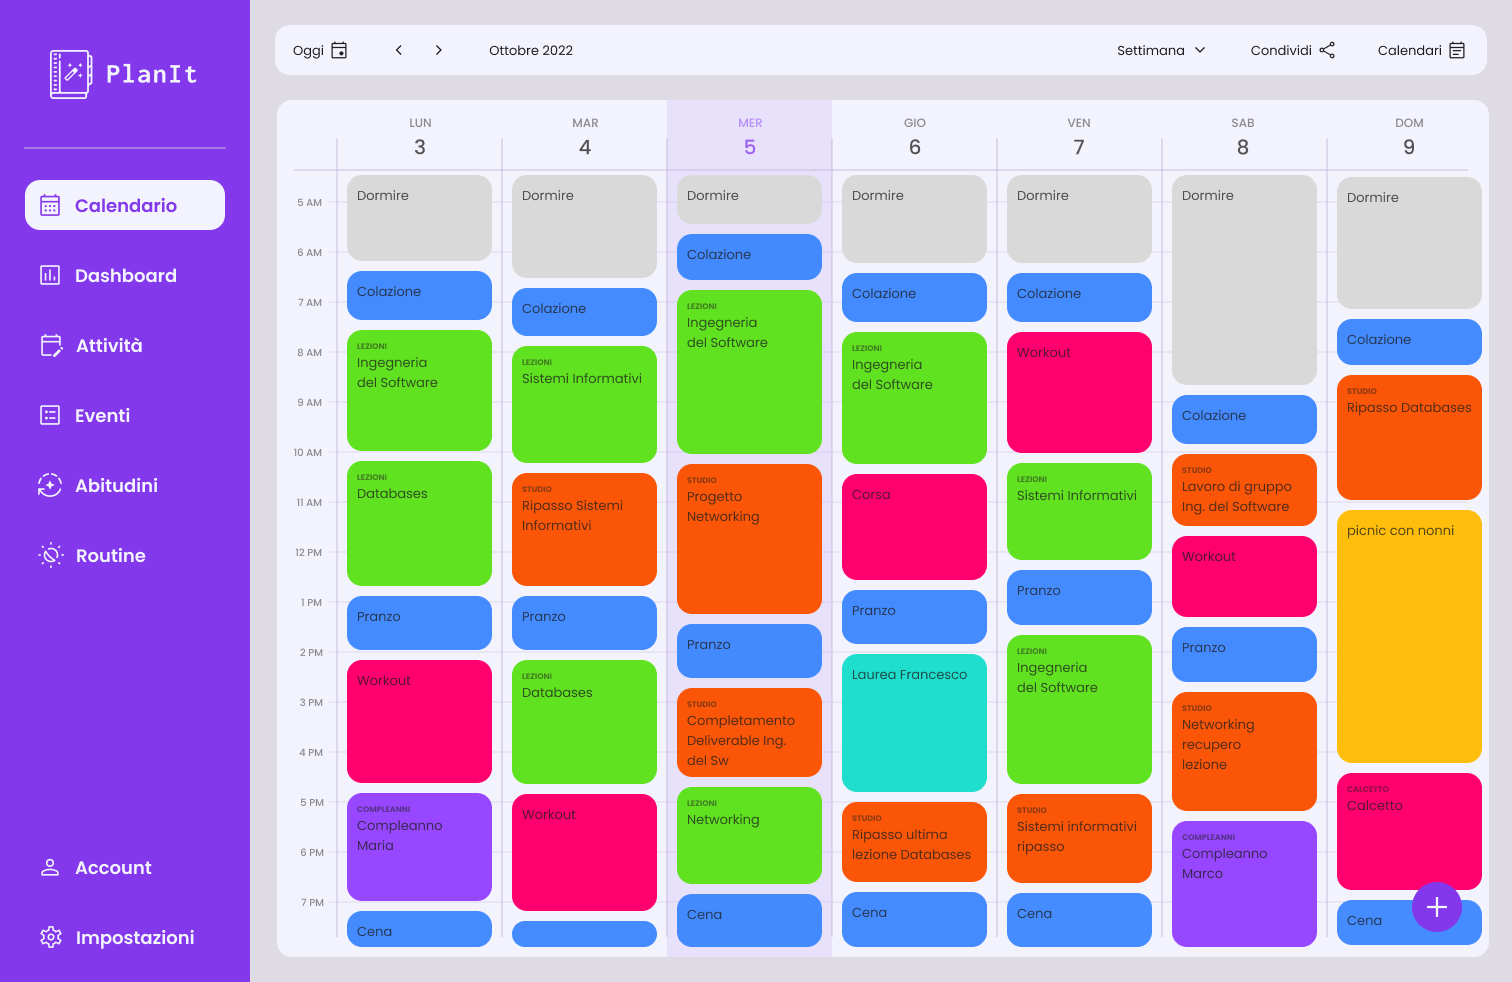
\includegraphics[width=1\textwidth]{img/FrontEnd/Calendar/Calendar.png}}
    \end{figure}
    
    \begin{listaPersonale2}{FE}
        \elemento[SCHERMATA PRINCIPALE-CALENDARI]{fe:2.1} Grazie alla sezione \href{https://www.figma.com/proto/cO66hx25OizBABGtWp8XlT/Planify?node-id=25%3A82&scaling=scale-down&page-id=0%3A1&starting-point-node-id=25%3A82}{"Calendari"}  l’utente aprirà una sezione da dove può gestire i propri calendari e i calendari condivisi di altre persone (\ref{rf:4.1}). I calendari condivisi da altri utenti sono indicati con una piccola immagine stereotipata di persone, alla destra del loro nome.
    \end{listaPersonale2}
    \begin{figure}[H]
        \centering
        \href{https://www.figma.com/proto/cO66hx25OizBABGtWp8XlT/Planify?node-id=25%3A82&scaling=scale-down&page-id=0%3A1&starting-point-node-id=25%3A82}{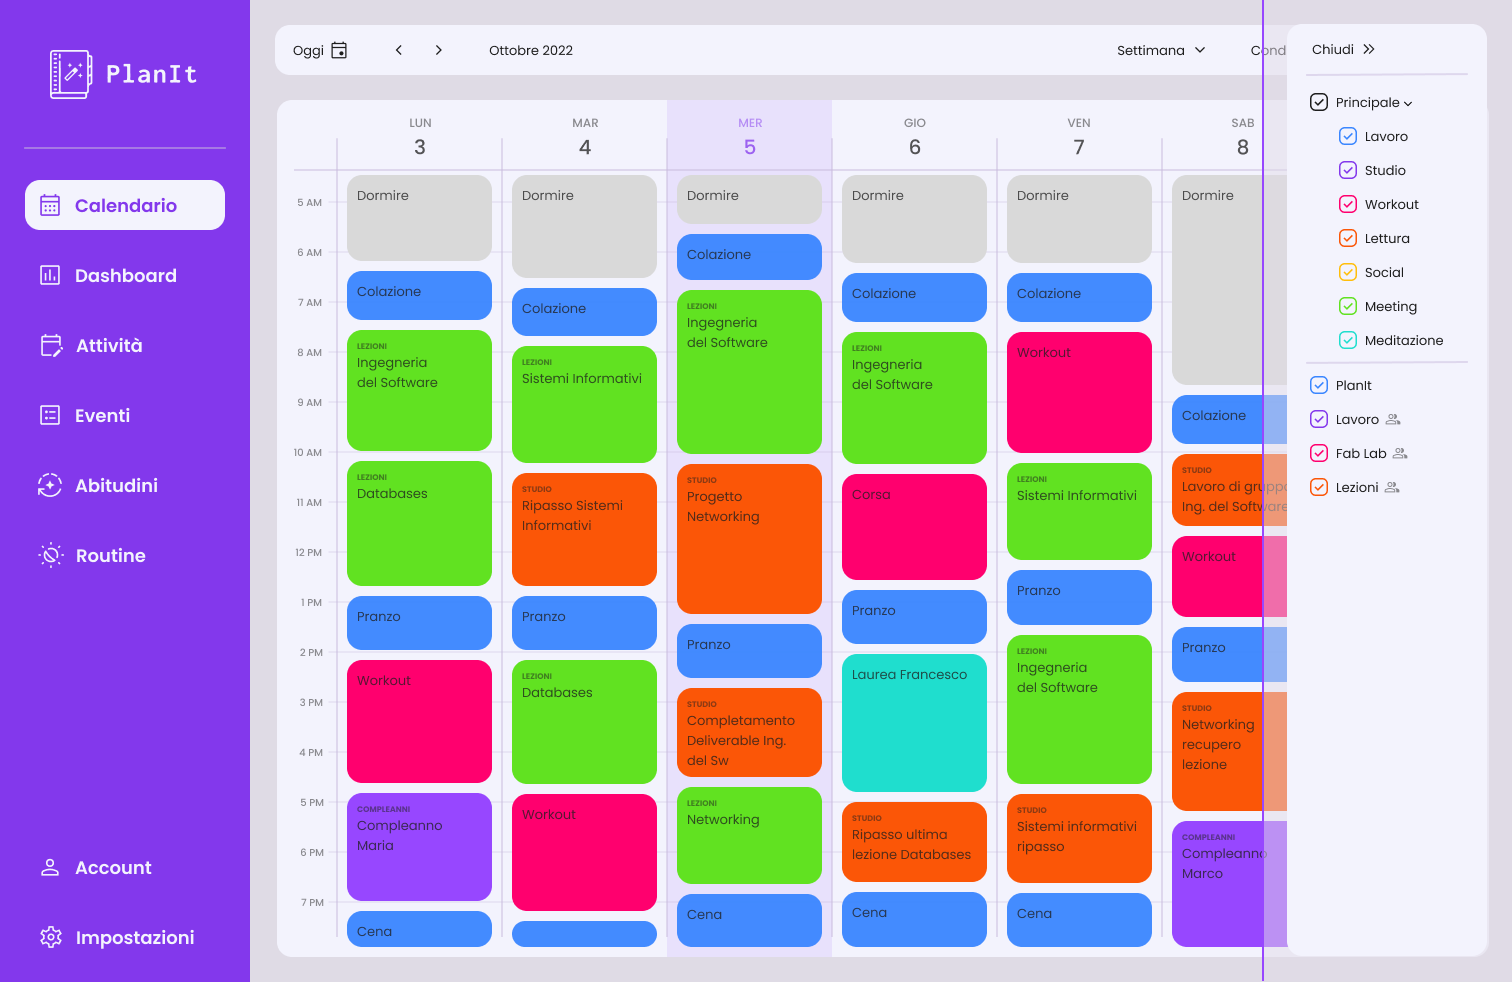
\includegraphics[width=0.9\textwidth,height=0.33\textheight]{img/FrontEnd/Calendar/CalendarCondivisi.png}}
    \end{figure}

    \pagebreak
    \elemento[DASHBOARD] {fe:3} L’utente, nella \href{https://www.figma.com/proto/cO66hx25OizBABGtWp8XlT/Planify?node-id=84%3A178&scaling=scale-down&page-id=0%3A1&starting-point-node-id=25%3A82}{dashboard}, può osservare le informazioni principali riguardo al proprio calendario, le sezioni presenti sono: "Attività svolte questa settimana", "Situazione scadenza attività" e "Attività svolte oggi" con "Grafico attività svolte".
    \begin{figure}[H]
        \centering
        \href{https://www.figma.com/proto/cO66hx25OizBABGtWp8XlT/Planify?node-id=84%3A178&scaling=scale-down&page-id=0%3A1&starting-point-node-id=25%3A82}{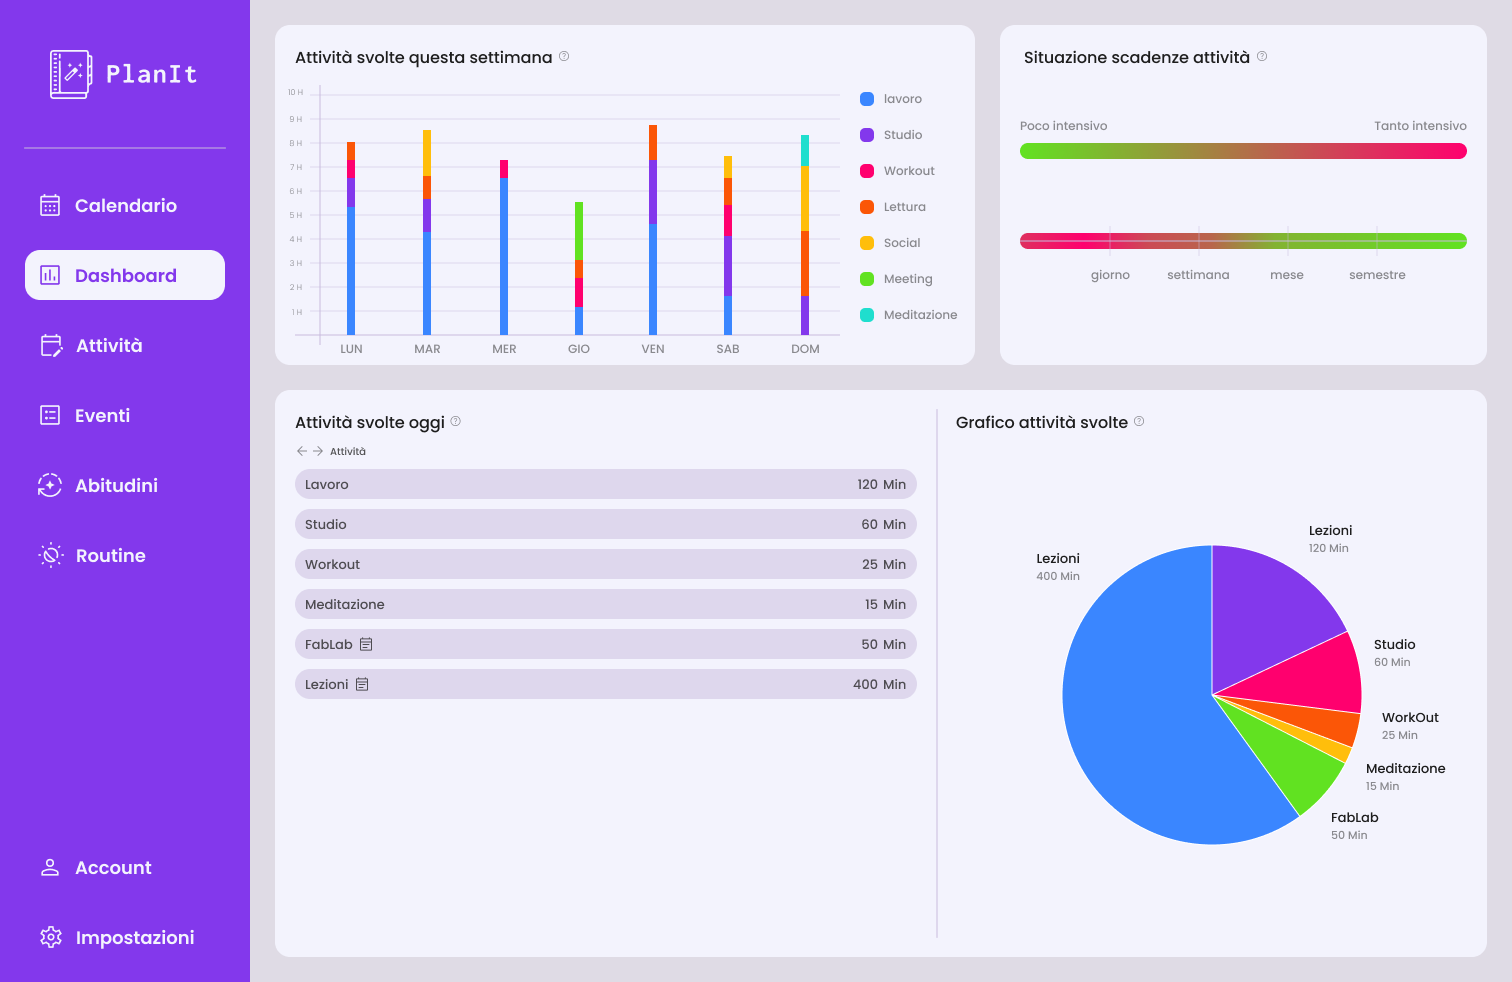
\includegraphics[width=1\textwidth]{img/FrontEnd/Dashboard/Dashboard.png}}
    \end{figure}

    
    \begin{listaPersonale2}{FE}
        \elemento[ATTIVITA' SVOLTE QUESTA SETTIMANA] {fe:3.1} Nella sezione “Attività svolte questa settimana” viene mostrato un grafico a barre delle varie attività svolte per ogni giorno della settimana (\ref{rf:9}); l’altezza delle barre corrisponde al quantitativo di ore dedicate a quell’attività.
        \begin{figure}[H]
            \centering
            \href{https://www.figma.com/proto/cO66hx25OizBABGtWp8XlT/Planify?node-id=84%3A178&scaling=scale-down&page-id=0%3A1&starting-point-node-id=25%3A82}{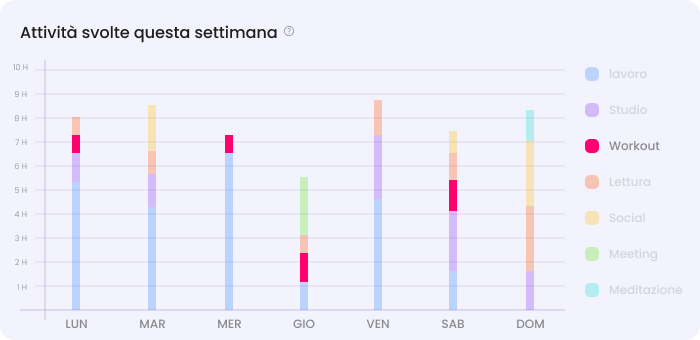
\includegraphics[width=0.6\textwidth,height=0.18\textheight]{img/FrontEnd/Dashboard/graficoBarre.png}}
            \caption{Figura 3.1: come appare il grafico quando si preme una delle attività della mia legenda}
        \end{figure}
        \pagebreak
        \elemento[SITUAZIONE SCADENZA ATTIVITA'] {fe:3.2}
        Nella sezione “Situazione scadenze attività” è presente in basso una heatmap riguardo al tempo che deve essere dedicato ogni giorno per rispettare le varie deadline (\ref{rf:9}). La legenda sopra la heatmap mostra che più si è tendenti al colore rosso, più ore si devono  impiegare nello specifico periodo di tempo.
        \begin{figure}[H]
            \centering
            \href{https://www.figma.com/proto/cO66hx25OizBABGtWp8XlT/Planify?node-id=84%3A178&scaling=scale-down&page-id=0%3A1&starting-point-node-id=25%3A82}{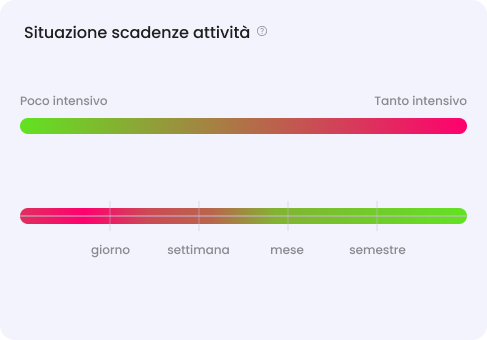
\includegraphics[width=0.45\textwidth,height=0.18\textheight]{img/FrontEnd/Dashboard/heatMap.png}}
        \end{figure}
        
        \elemento [ATTIVITA’ SVOLTE OGGI e GRAFICO ATTIVITA' SVOLTE] {fe:3.3} Nella sezione “Attività svolte oggi” è presente una lista delle attività della giornata, da cui si possono ottenere anche le varie sottoattività. 
        La sezione “Attività svolte oggi” è sincronizzata con il grafico a torta presente nel “Grafico attività svolte” (\ref{rf:9}). Il grafico presenta le attività selezionate in “Attività svolte oggi” con una dimensione proporzionata al tempo da spendere.

        \begin{figure}[H]
            \centering
            \href{https://www.figma.com/proto/cO66hx25OizBABGtWp8XlT/Planify?node-id=84%3A178&scaling=scale-down&page-id=0%3A1&starting-point-node-id=25%3A82}{\includegraphics[width=0.72\textwidth,height=0.2\textheight]{img/FrontEnd/Dashboard/selezionatoAttività.png}}
            \caption{Figura 3.3.1: schermata che appare quando si mette il puntatore sopra una delle raggruppamenti della lista}
        \end{figure}

        \begin{figure}[H]
            \centering
            \href{https://www.figma.com/proto/cO66hx25OizBABGtWp8XlT/Planify?node-id=84%3A178&scaling=scale-down&page-id=0%3A1&starting-point-node-id=25%3A82}{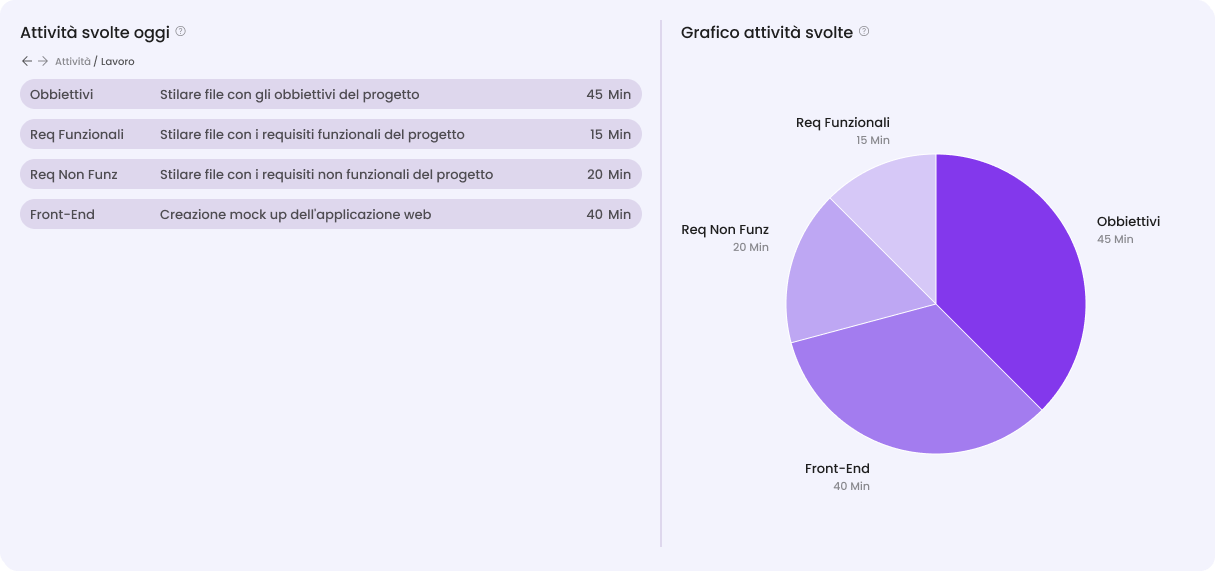
\includegraphics[width=0.72\textwidth,height=0.2\textheight]{img/FrontEnd/Dashboard/Dashboard3.png}}
            \caption{Figura 3.3.2: schermata quando si seleziona una delle attività della lista}
        \end{figure}
           
    \end{listaPersonale2}
    \pagebreak
    \elemento [SCHERMATA ATTIVITA'] {fe:4} Nella \href{https://www.figma.com/proto/cO66hx25OizBABGtWp8XlT/Planify?node-id=159%3A277&scaling=scale-down&page-id=0%3A1&starting-point-node-id=25%3A82}{schermata attività} è presente una tabella delle attività della giornata con le varie informazioni, ovvero: titolo, descrizione, categoria, priorità, durata (\ref{rf:5}), posizione (\ref{rf:8.2}) e difficoltà. Inoltre ci sono dei tasti con cui si può ritardare (\ref{rf:10}), eliminare (\ref{rf:5})l'attività e, infine, un tasto per indicare di averla completata. A fine giornata di default tutti gli impegni sono posti come completati; per modificare tale opzione deve intervenire l’utente.
    \begin{figure}[H]
        \centering
        \href{https://www.figma.com/proto/cO66hx25OizBABGtWp8XlT/Planify?node-id=159%3A277&scaling=scale-down&page-id=0%3A1&starting-point-node-id=25%3A82}{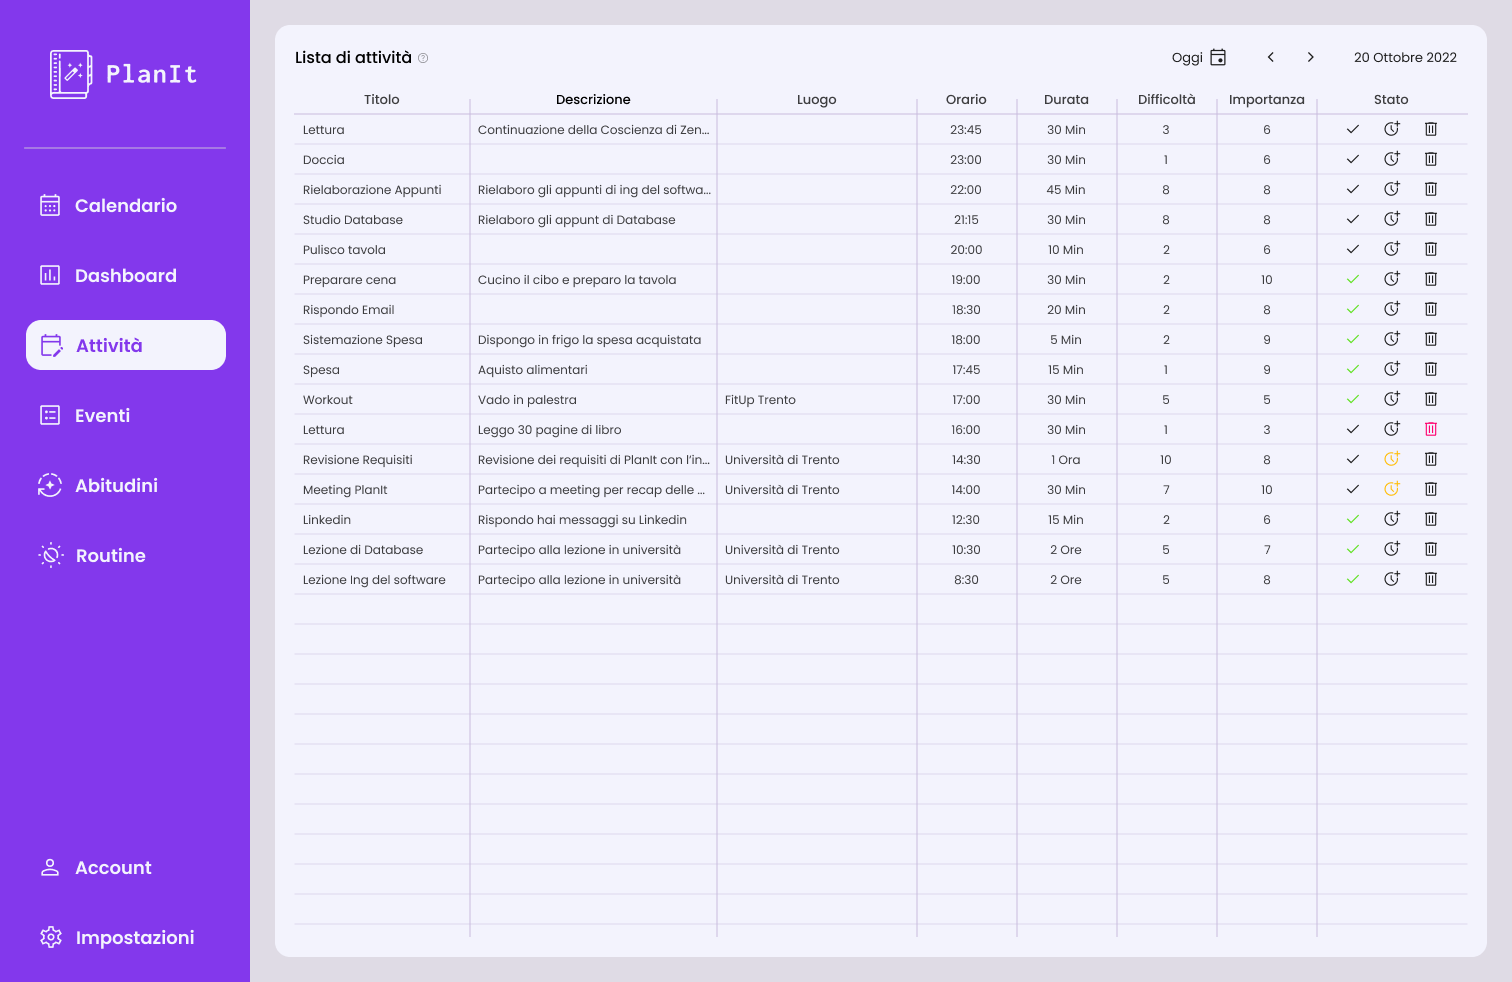
\includegraphics[width=1\textwidth]{img/FrontEnd/Attivita/Attivita.png}}
        \caption {Figura 4: le spunte verdi indicano il completamento dell'evento; l'orologio giallo indica il ritardo nel compiere l'evento; il cestino l'eliminazione dell'evento}
    \end{figure}
    \pagebreak
    \elemento [SCHERMATA EVENTI] {fe:5} Nella \href{https://www.figma.com/proto/cO66hx25OizBABGtWp8XlT/Planify?node-id=160%3A290&scaling=scale-down&page-id=0%3A1&starting-point-node-id=25%3A82}{schermata eventi} sono presenti tutti i comandi che riguardano la compilazione ed eliminazione di eventi (\ref{rf:5}), calendari (\ref{rf:4.2}) e raggruppamenti (RF\ref{rf:5.9}).
    Nella sezione sottostante, è presente una lista dei vari calendari, eventi e raggruppamenti, che selezionati una alla volta aprono i rispettivi form di modifica, dove sono presenti tutti i campi citati in (\ref{rf:5}) per l’aggiunta e modifica di impegni e raggruppamenti e (\ref{rf:13}) per la modifica e aggiunta di calendari. Mediante un'azione di "drag and drop" è possibile spostare l'elemento selezionato da una posizione all'altra della lista.
    %qua dipende dalla formattazione andrebbe un clearpage
    \begin{figure}[H]
        \centering
        \href{https://www.figma.com/proto/cO66hx25OizBABGtWp8XlT/Planify?node-id=160%3A290&scaling=scale-down&page-id=0%3A1&starting-point-node-id=25%3A82}{\includegraphics[width=1\textwidth]{img/FrontEnd/Eventi/SottoAttività.png}}
        \caption{Figura 5: schermata quando si apre la sezione "Eventi"}
    \end{figure}
    \begin{figure}[H]
        \centering
        \href{https://www.figma.com/proto/cO66hx25OizBABGtWp8XlT/Planify?node-id=160%3A290&scaling=scale-down&page-id=0%3A1&starting-point-node-id=25%3A82}{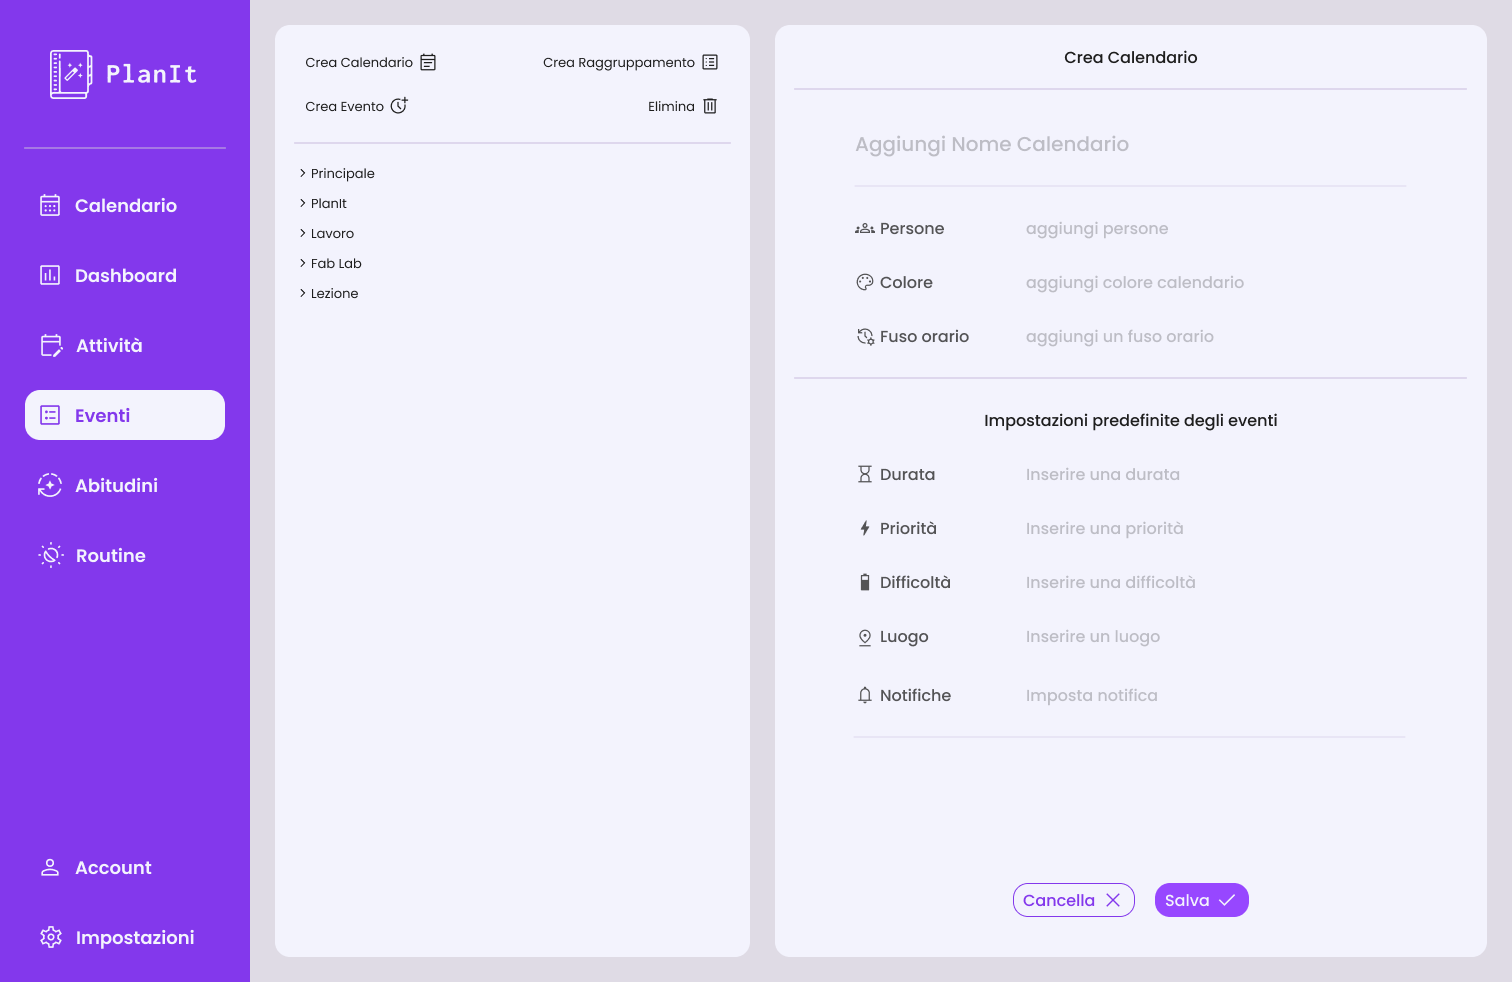
\includegraphics[width=1\textwidth]{img/FrontEnd/Eventi/Calendario/CreaCalendario.png}}
        \caption{Figura 5: schermata quando si seleziona uno dei comandi o un'attività della lista}
    \end{figure}
    \begin{listaPersonale2}{FE}
        
        \elemento[SCHERMATA CREA/MODIFICA EVENTO] {fe:5.1}

        \begin{center} 
            \begin{figure}[H]
            \centering        
            \href{https://www.figma.com/proto/cO66hx25OizBABGtWp8XlT/Planify?node-id=160%3A290&scaling=scale-down&page-id=0%3A1&starting-point-node-id=25%3A82}{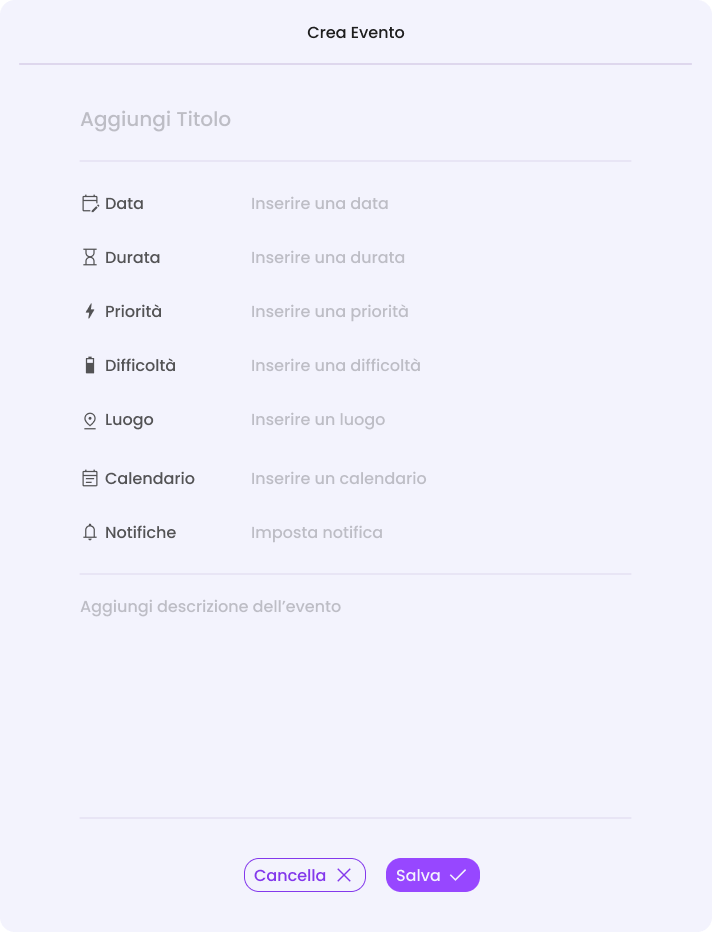
\includegraphics[width=0.49\textwidth,height=0.35\textheight]{img/FrontEnd/Eventi/Evento/CreaEvento.png}}
            \centering
            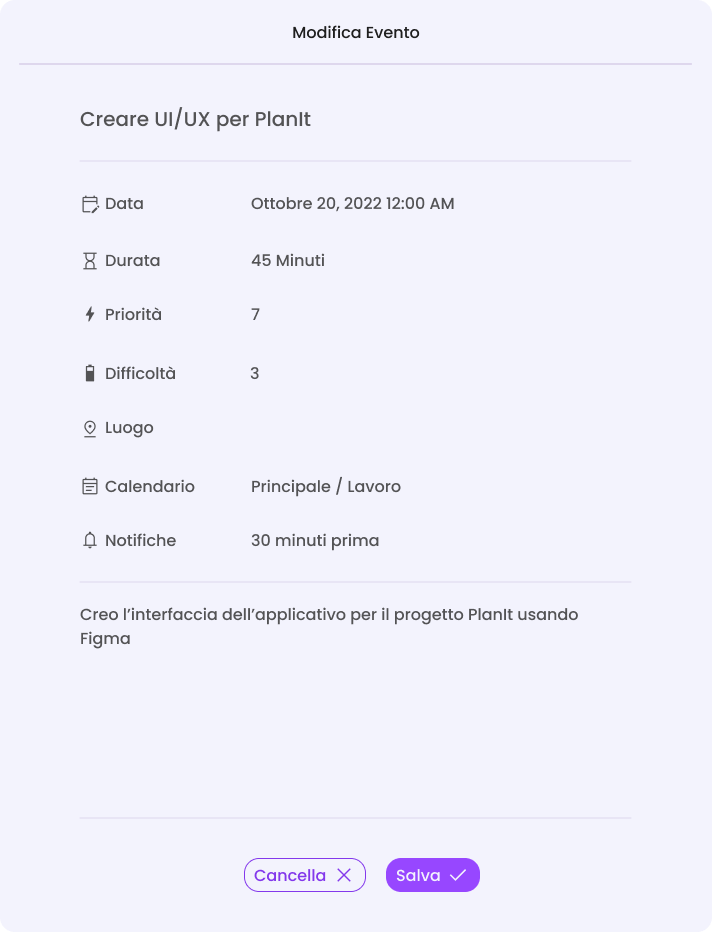
\includegraphics[width=0.49\textwidth,height=0.35\textheight]{img/FrontEnd/Eventi/Evento/ModificaEvento.png}
            \end{figure}
        \end{center}

        
        \elemento[SCHERMATA CREA/MODIFICA RAGGRUPPAMENTO] {fe:5.2}

        \begin{center} 
            \begin{figure}[H]
            \centering
            \href{https://www.figma.com/proto/cO66hx25OizBABGtWp8XlT/Planify?node-id=160%3A290&scaling=scale-down&page-id=0%3A1&starting-point-node-id=25%3A82}{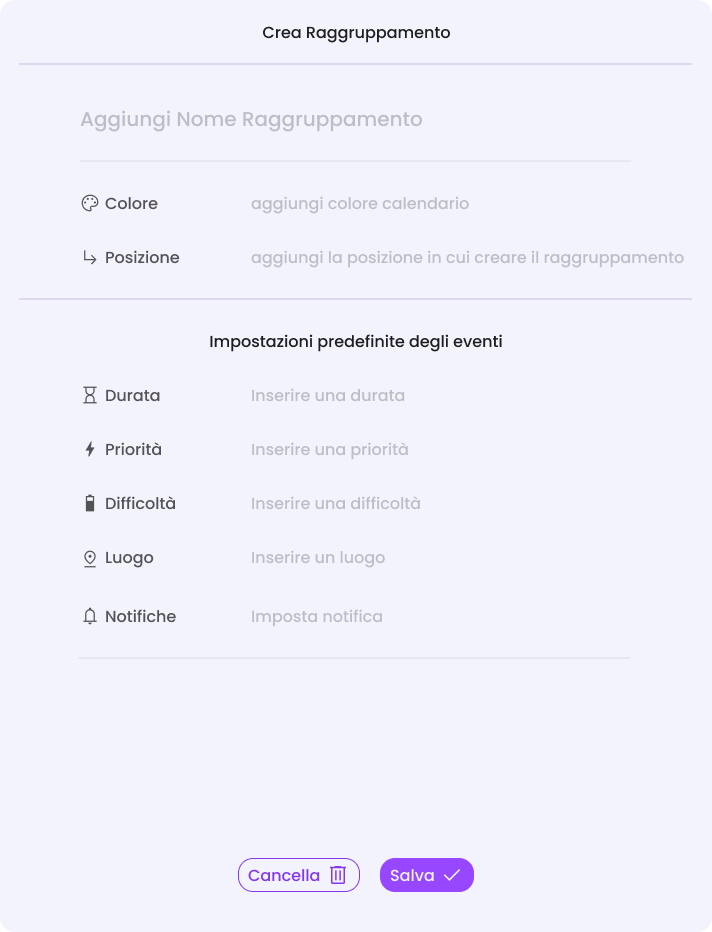
\includegraphics[width=0.49\textwidth,height=0.35\textheight]{img/FrontEnd/Eventi/Raggruppamento/CreaRaggruppamento.png}}
            \centering
            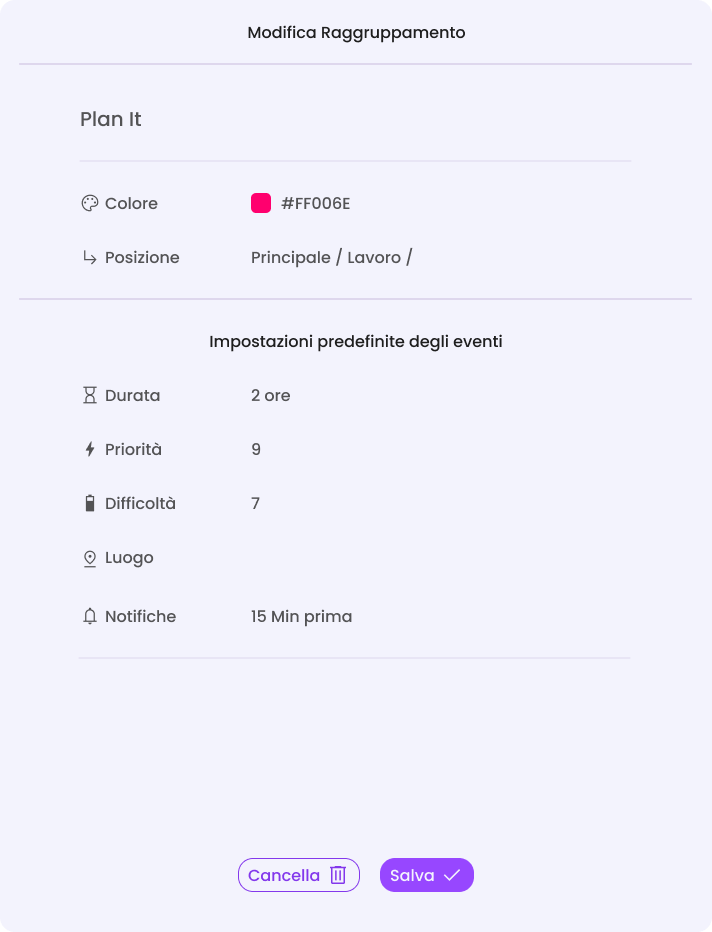
\includegraphics[width=0.49\textwidth,height=0.35\textheight]{img/FrontEnd/Eventi/Raggruppamento/ModificaRaggruppamento.png}
            \end{figure}
        \end{center}
        \pagebreak
        \elemento[SCHERMATA CREA/MODIFICA CALENDARIO] {fe:5.3}

        \begin{center} 
            \begin{figure}[H]
            \centering
            \href{https://www.figma.com/proto/cO66hx25OizBABGtWp8XlT/Planify?node-id=160%3A290&scaling=scale-down&page-id=0%3A1&starting-point-node-id=25%3A82}{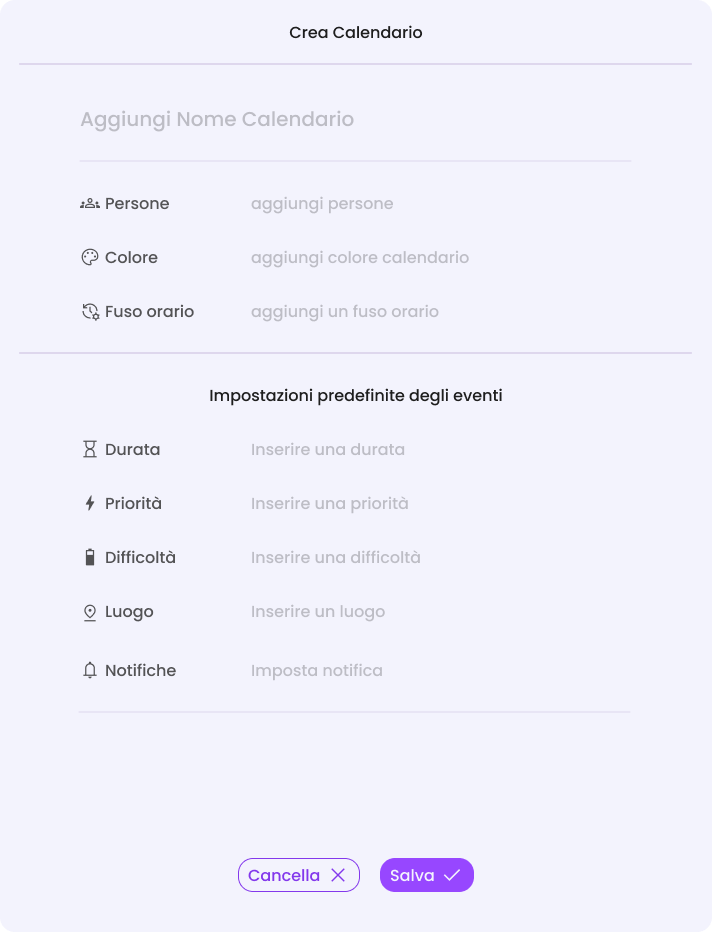
\includegraphics[width=0.49\textwidth,height=0.35\textheight]{img/FrontEnd/Eventi/Calendario/CreaCalendario1.png}}
            \centering
            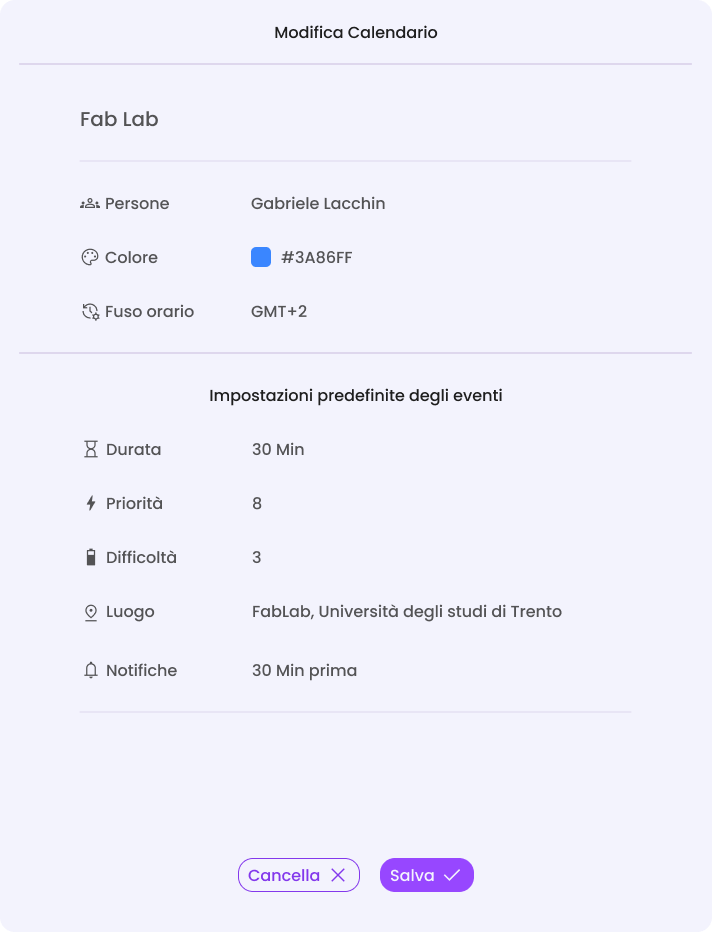
\includegraphics[width=0.49\textwidth,height=0.35\textheight]{img/FrontEnd/Eventi/Calendario/ModificaCalendario.png}
            \end{figure}
        \end{center}
        
    \end{listaPersonale2}
    \pagebreak
    \elemento [SCHERMATA ABITUDINI] {fe:6} Nella schermata          \href{https://www.figma.com/proto/cO66hx25OizBABGtWp8XlT/Planify?node-id=160%3A399&scaling=scale-down&page-id=0%3A1&starting-point-node-id=25%3A82}{"Abitudini"} l’utente può visualizzare la lista delle abitudini del proprio calendario. Inoltre, nella sezione di destra, si può aprire un form per la modifica, aggiunta ed eliminazione (\ref{rf:5}) di un'abitudine(RF\ref{rf:5.4}) selezionando una di quest'ultime.
    \begin{figure}[H]
        \centering
        \href{https://www.figma.com/proto/cO66hx25OizBABGtWp8XlT/Planify?node-id=160%3A399&scaling=scale-down&page-id=0%3A1&starting-point-node-id=25%3A82}{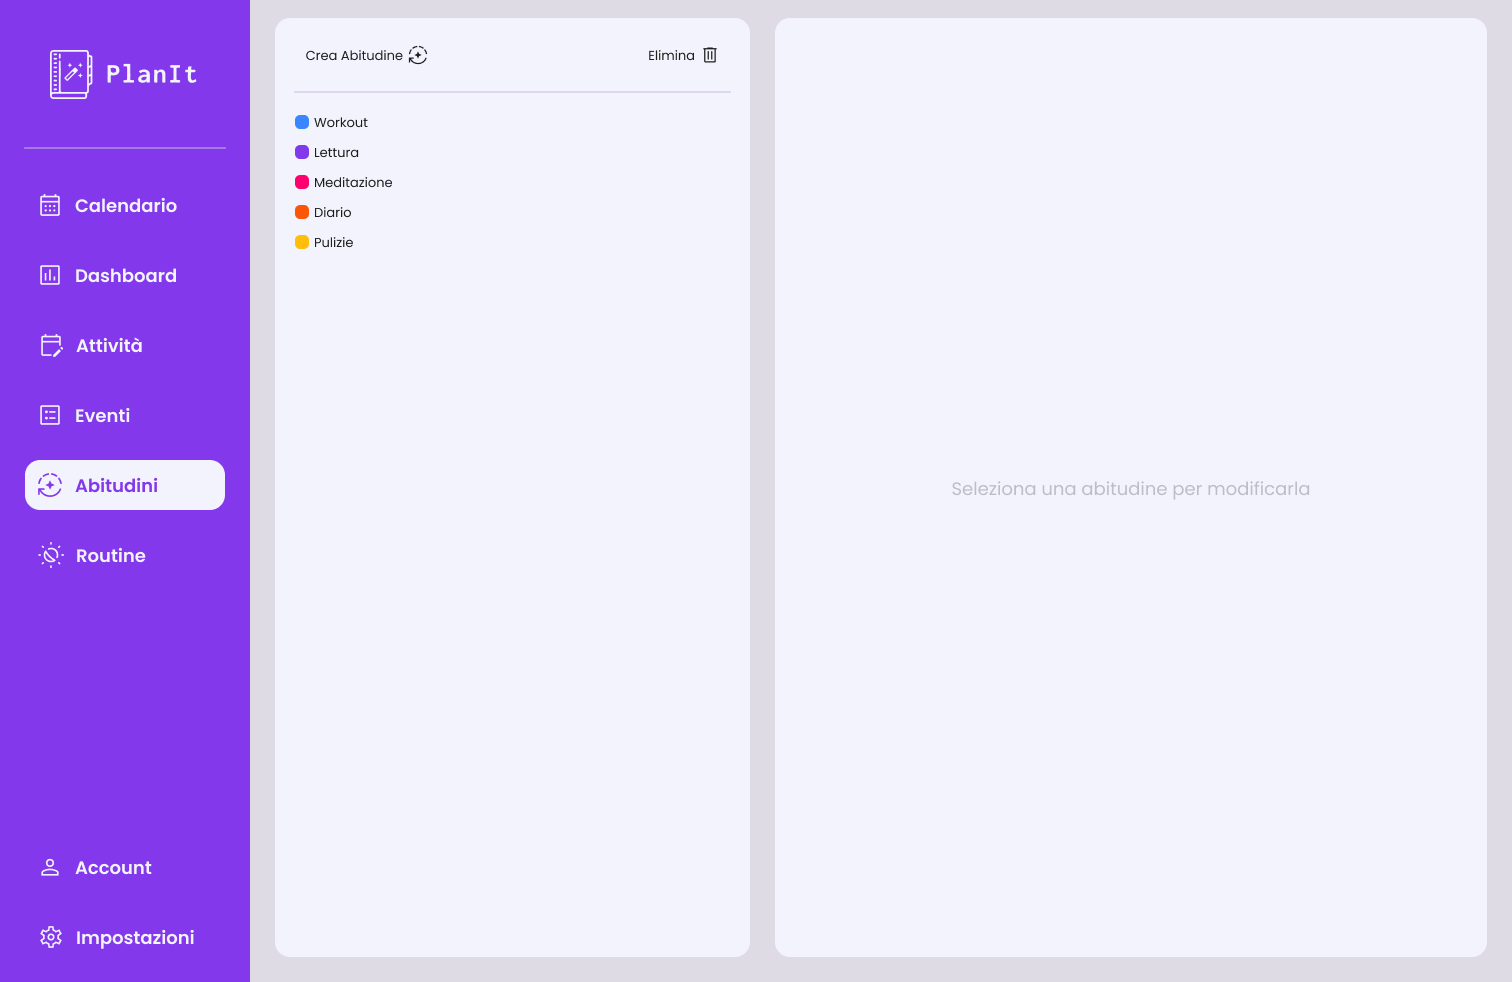
\includegraphics[width=1\textwidth]{img/FrontEnd/Abitudini/Abitudini.png}}
        \caption{Figura 6: schermata quando si apre la sezione "Abitudini"}
    \end{figure}

    \begin{figure}[H]
        \centering
        \href{https://www.figma.com/proto/cO66hx25OizBABGtWp8XlT/Planify?node-id=160%3A399&scaling=scale-down&page-id=0%3A1&starting-point-node-id=25%3A82}{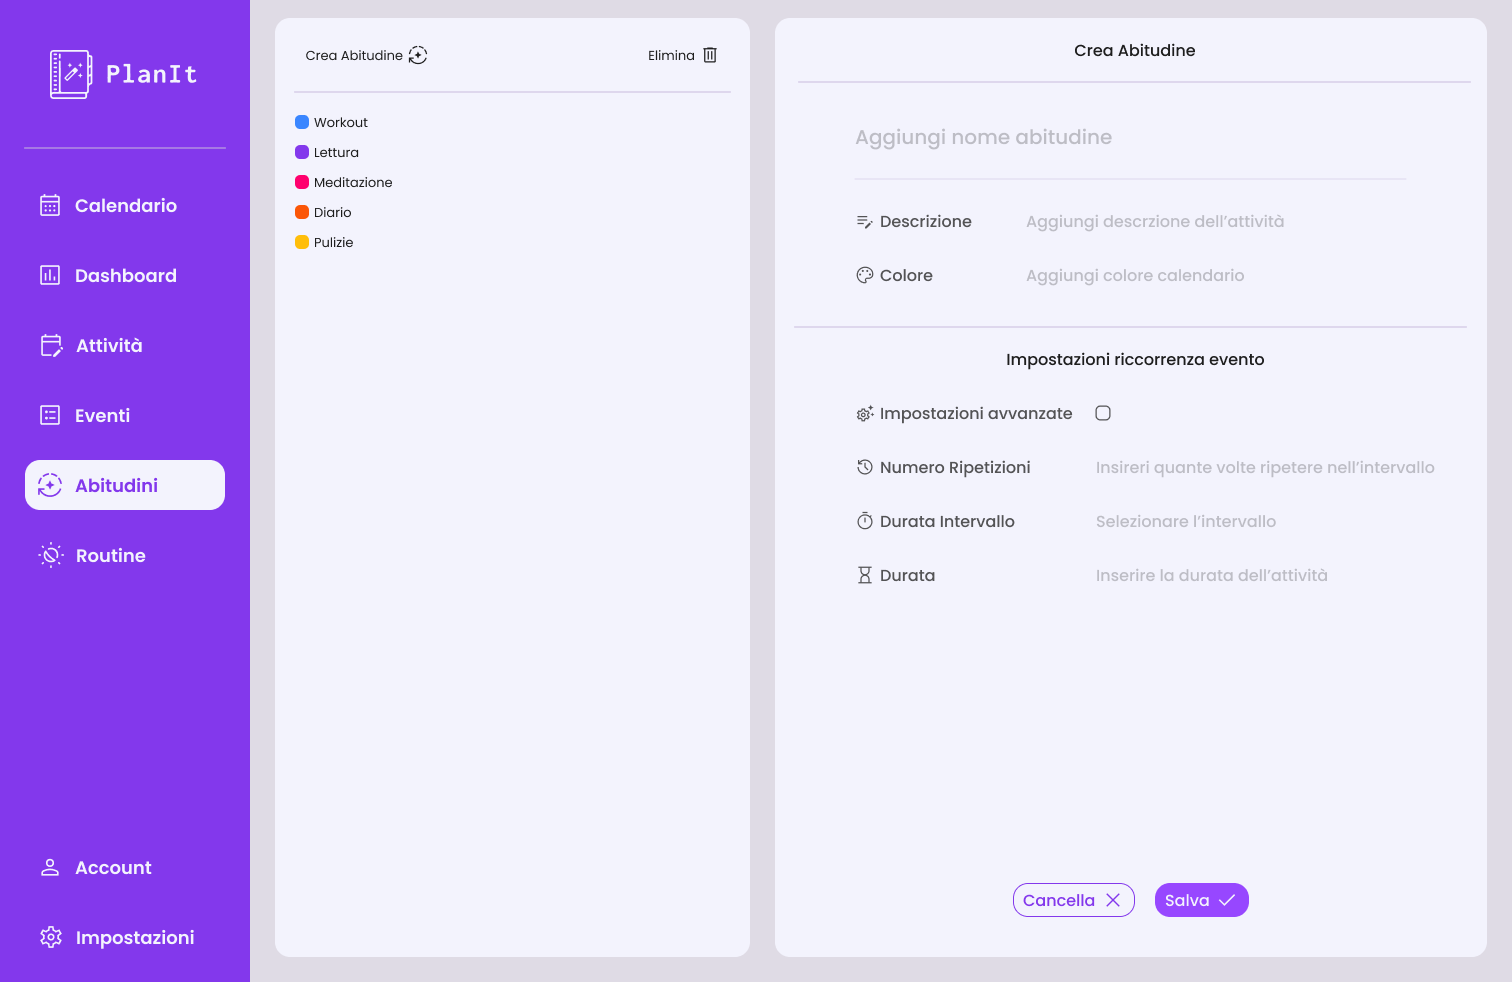
\includegraphics[width=1\textwidth]{img/FrontEnd/Abitudini/CreaAbitudiniMain.png}}
        \caption{Figura 6: schermata quando si seleziona uno dei comandi o un'abitudine della lista}
    \end{figure}

    \begin{listaPersonale2}{FE}
        
        \elemento[SCHERMATA CREA ABITUDINI E IMPOSTAZIONI AVANZATE]{fe:6.1}
        \begin{center} 
            \begin{figure}[H]
            \centering
            \href{https://www.figma.com/proto/cO66hx25OizBABGtWp8XlT/Planify?node-id=160%3A399&scaling=scale-down&page-id=0%3A1&starting-point-node-id=25%3A82}{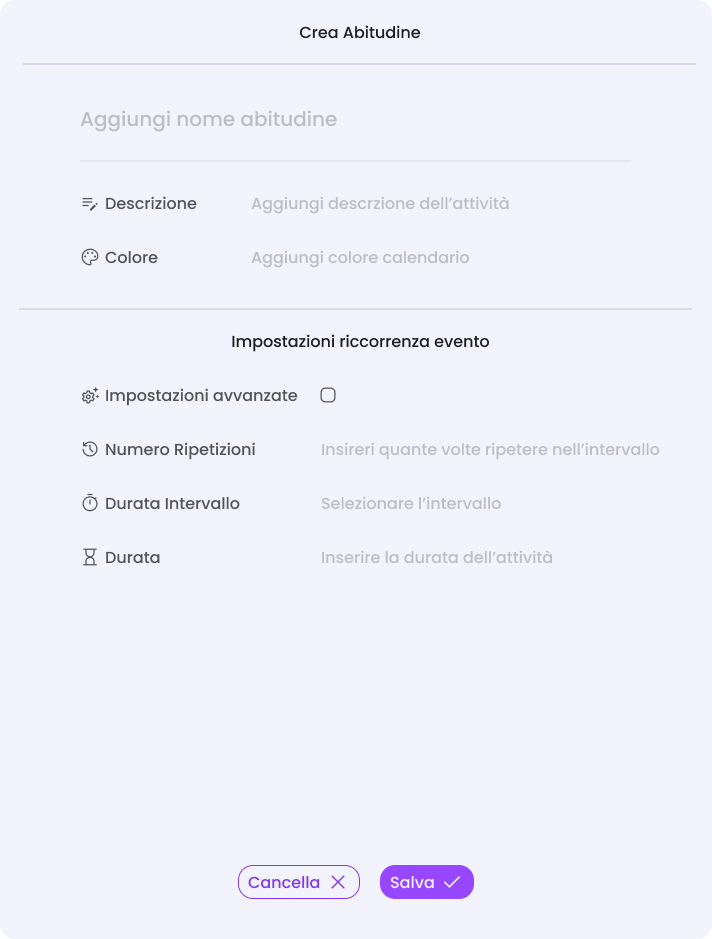
\includegraphics[width=0.49\textwidth,height=0.35\textheight]{img/FrontEnd/Abitudini/Crea/CreaAbitudine.png}}
            \centering
            \href{https://www.figma.com/proto/cO66hx25OizBABGtWp8XlT/Planify?node-id=160%3A399&scaling=scale-down&page-id=0%3A1&starting-point-node-id=25%3A82}{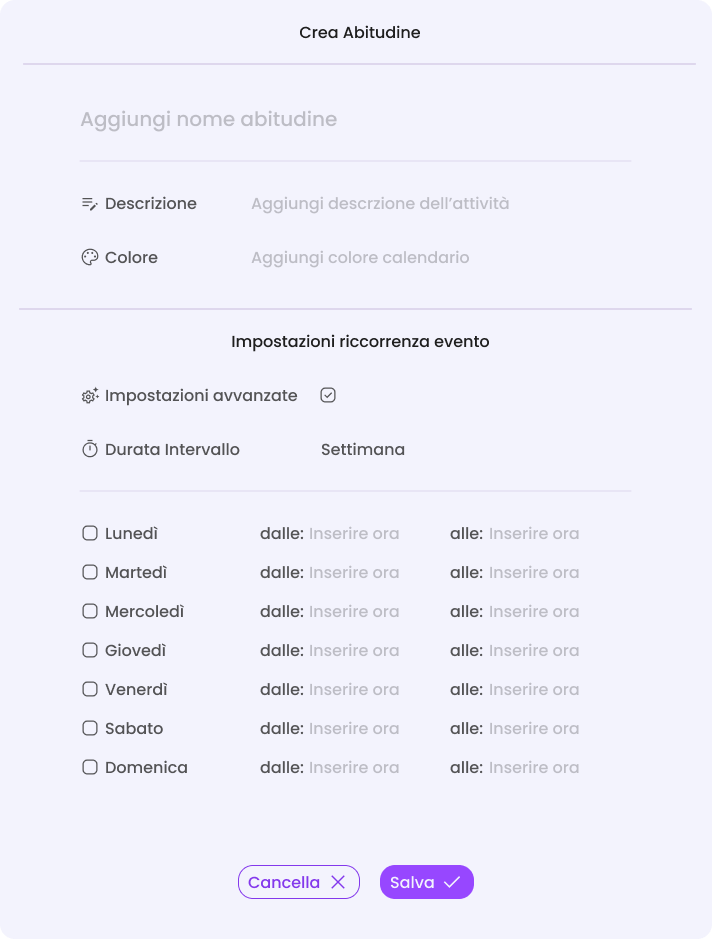
\includegraphics[width=0.49\textwidth,height=0.35\textheight]{img/FrontEnd/Abitudini/Crea/CreaAbitudineAvv.png}}
            \end{figure}
        \end{center}

        \elemento [SCHERMATA MODIFICA ABITUDINI E IMPOSTAZIONI AVANZATE] {fe:6.2}
        \begin{center} 
            \begin{figure}[H]
            \centering
            \href{https://www.figma.com/proto/cO66hx25OizBABGtWp8XlT/Planify?node-id=160%3A399&scaling=scale-down&page-id=0%3A1&starting-point-node-id=25%3A82}{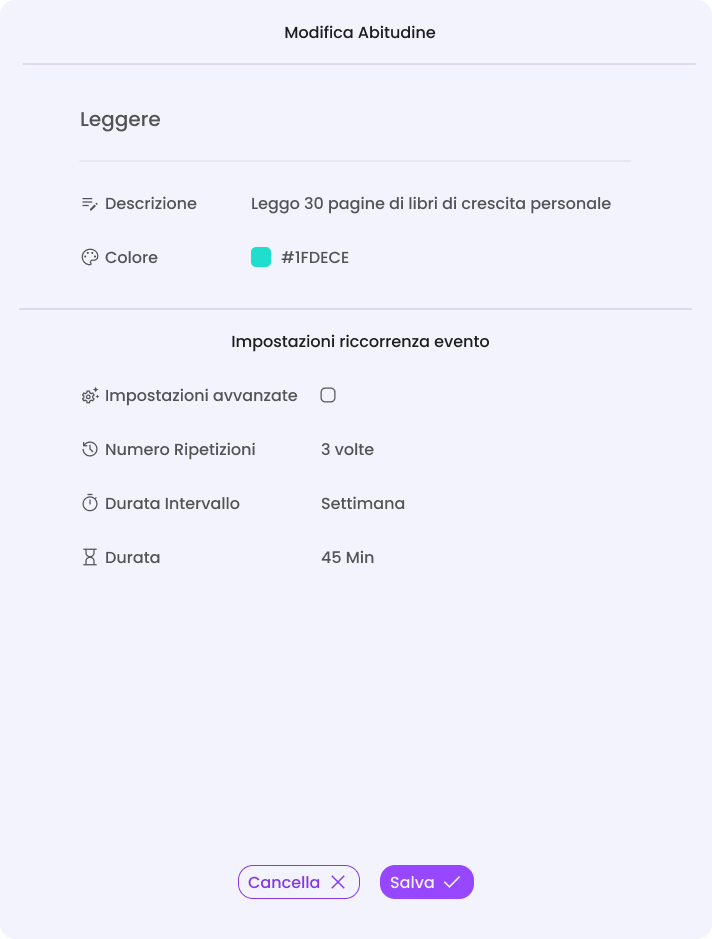
\includegraphics[width=0.49\textwidth,height=0.35\textheight]{img/FrontEnd/Abitudini/Modifica/ModificaAbitudine.png}}
            \centering
            \href{https://www.figma.com/proto/cO66hx25OizBABGtWp8XlT/Planify?node-id=160%3A399&scaling=scale-down&page-id=0%3A1&starting-point-node-id=25%3A82}{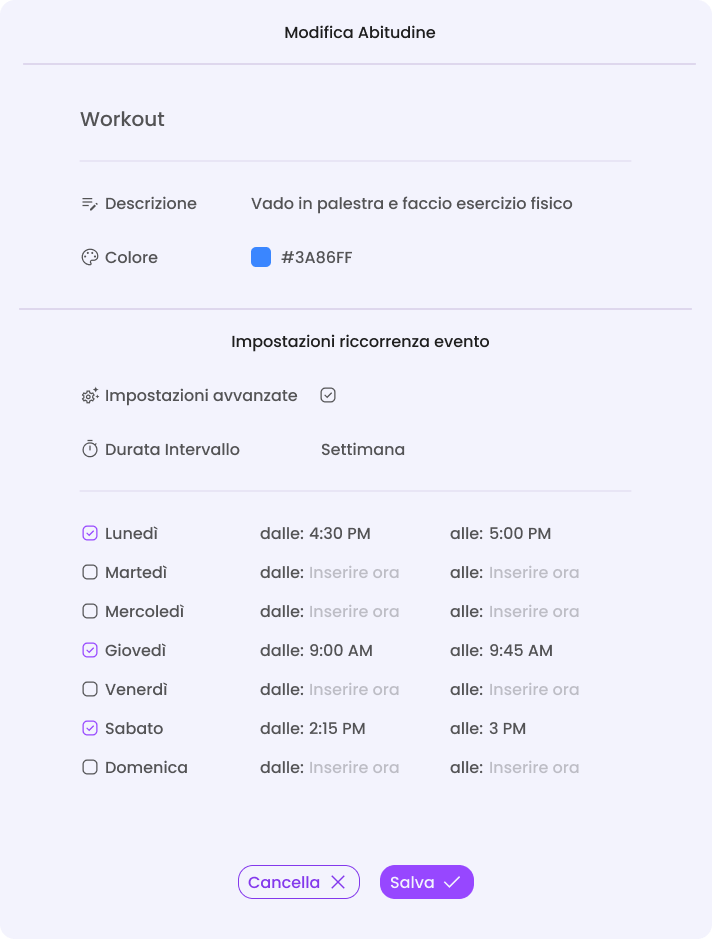
\includegraphics[width=0.49\textwidth,height=0.35\textheight]{img/FrontEnd/Abitudini/Modifica/ModificaAbitudineAvv.png}}
            \end{figure}
        \end{center}

    \end{listaPersonale2}
    \pagebreak
    \elemento [SCHERMATA ROUTINE] {fe:7} Nella schermata \href{https://www.figma.com/proto/cO66hx25OizBABGtWp8XlT/Planify?node-id=160%3A531&scaling=scale-down&page-id=0%3A1&starting-point-node-id=25%3A82}{“Routine”} l’utente ha possibilità di visualizzare e gestire tutte le proprie routine, ovvero le attività che ripete tutti i giorni (RF\ref{rf:5.5}), come dormire e mangiare. L’utente ha la possibilità di definire quante ore e quando avere queste attività di routine. L'utente può aggiungere le attività di routine da "Blocchi di attività" mediante un'azione di "drag and drop" nel tabella settimanale.
    \begin{figure}[H]
        \centering
        \href{https://www.figma.com/proto/cO66hx25OizBABGtWp8XlT/Planify?node-id=160%3A531&scaling=scale-down&page-id=0%3A1&starting-point-node-id=25%3A82}{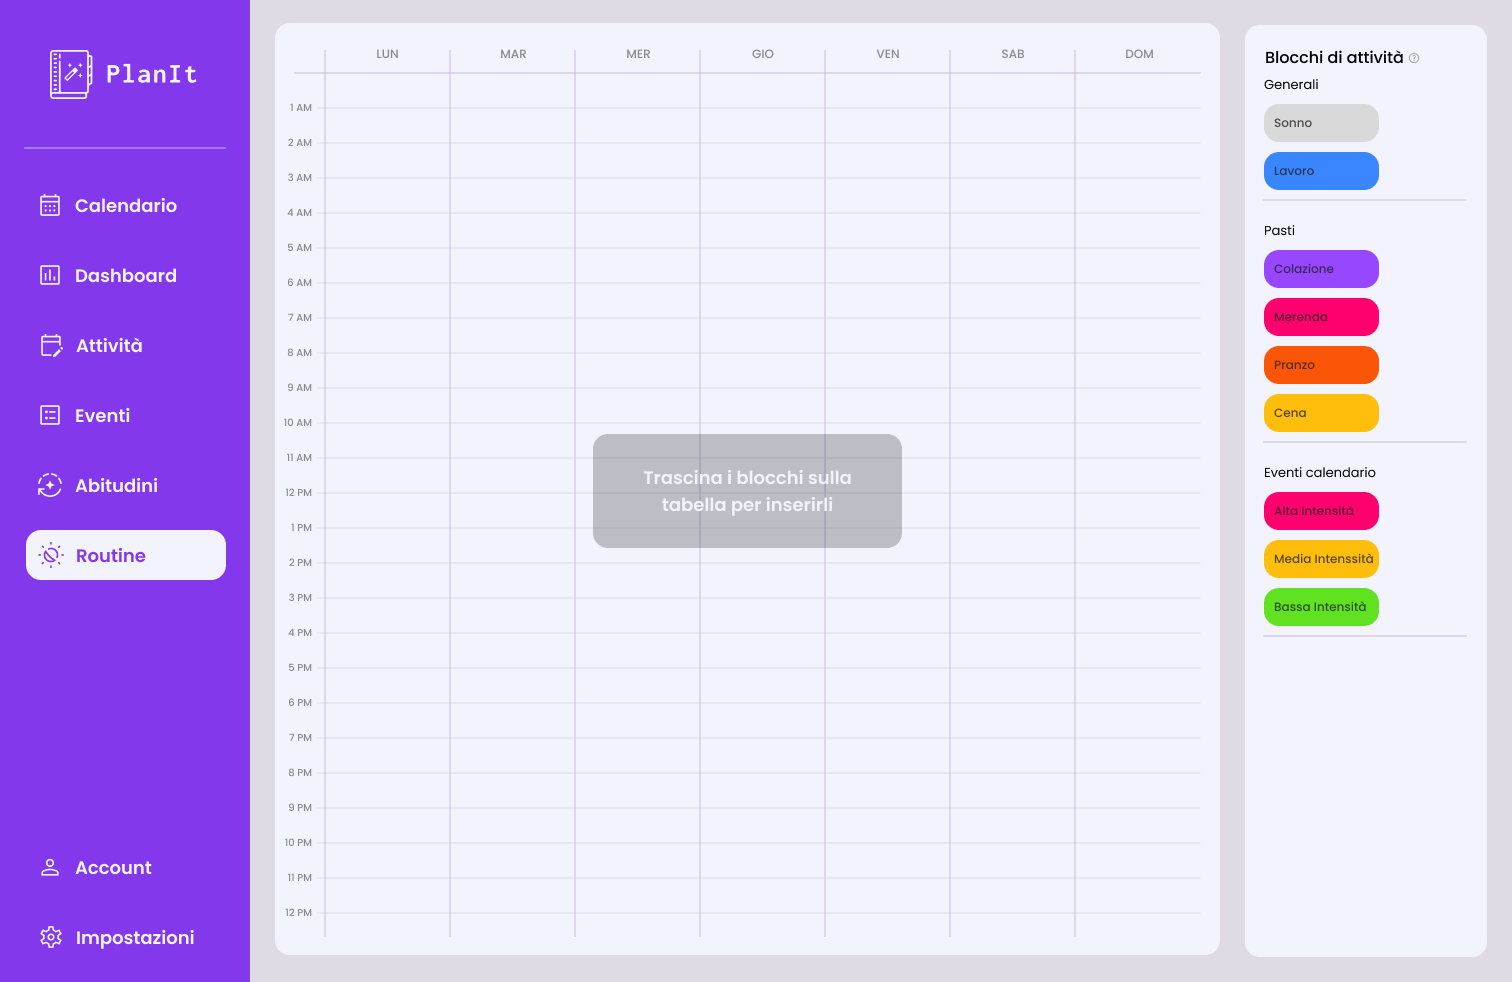
\includegraphics[width=1\textwidth]{img/FrontEnd/Routine/Routine.png}}
        \caption{Figura 7: schermata quando si apre la sezione "Routine"}
    \end{figure}
    \begin{figure}[H]
        \centering
        \href{https://www.figma.com/proto/cO66hx25OizBABGtWp8XlT/Planify?node-id=453%3A1711&scaling=scale-down&page-id=0%3A1&starting-point-node-id=25%3A82}{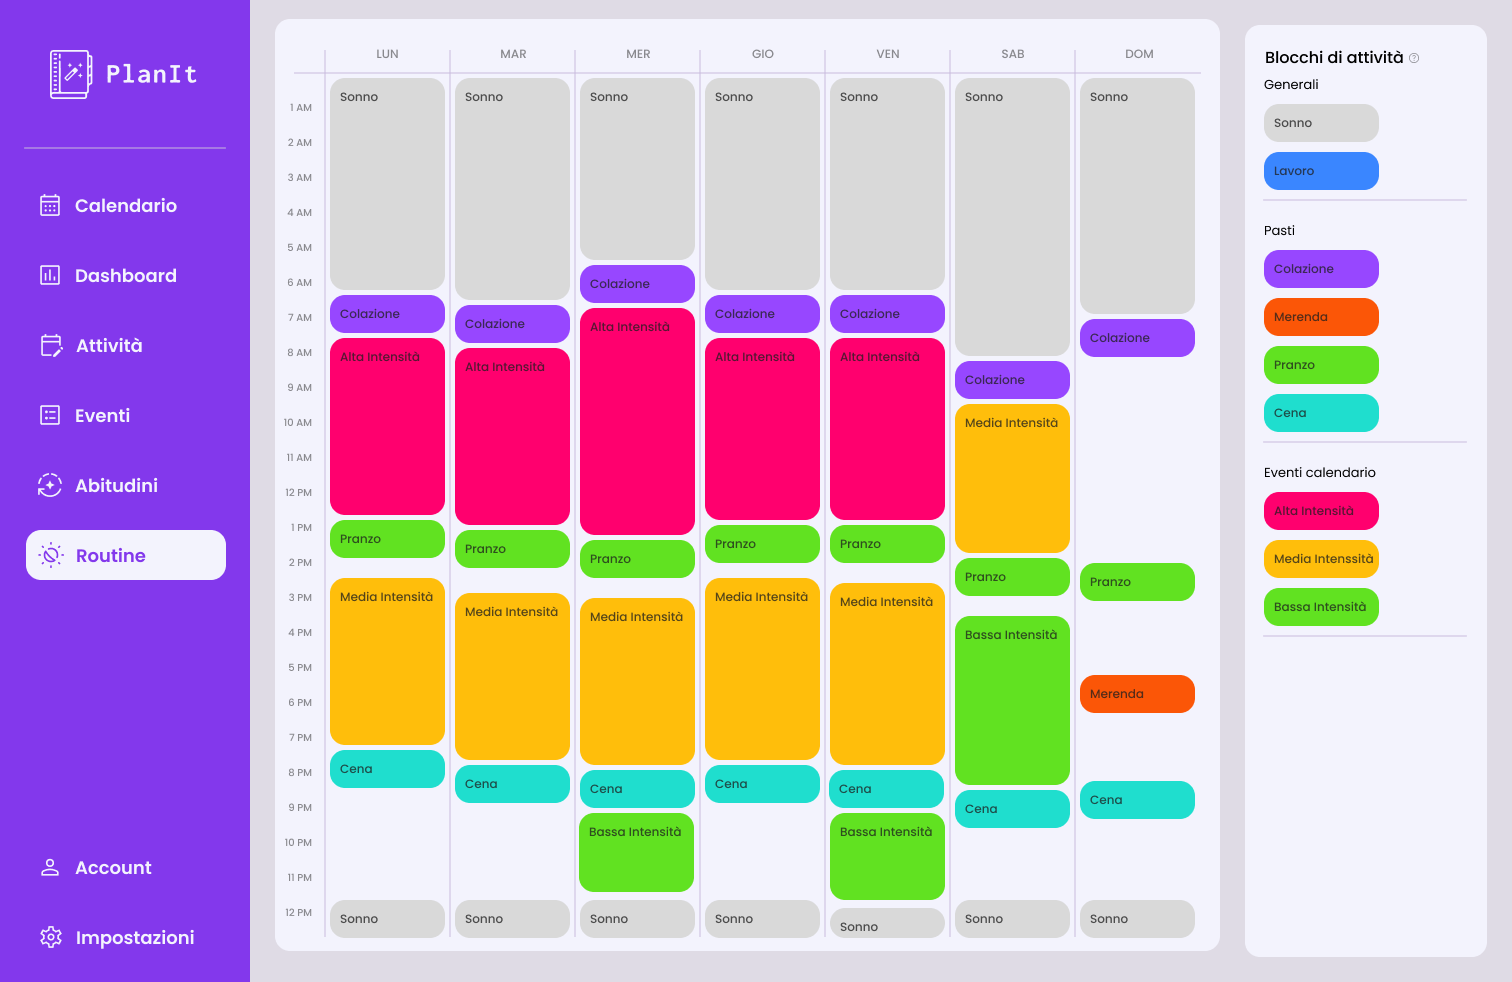
\includegraphics[width=1\textwidth]{img/FrontEnd/Routine/RoutineRiempito.png}}
        \caption{Figura 7.1: schermata quando si riempe il calendario settimanale con le routine mediante l'azione di "drag and drop"}
    \end{figure}
    

\end{listaPersonale}